\chapter{Arquitectura futura SWAT+ IGP}
\begin{figure}[htbp]\centering
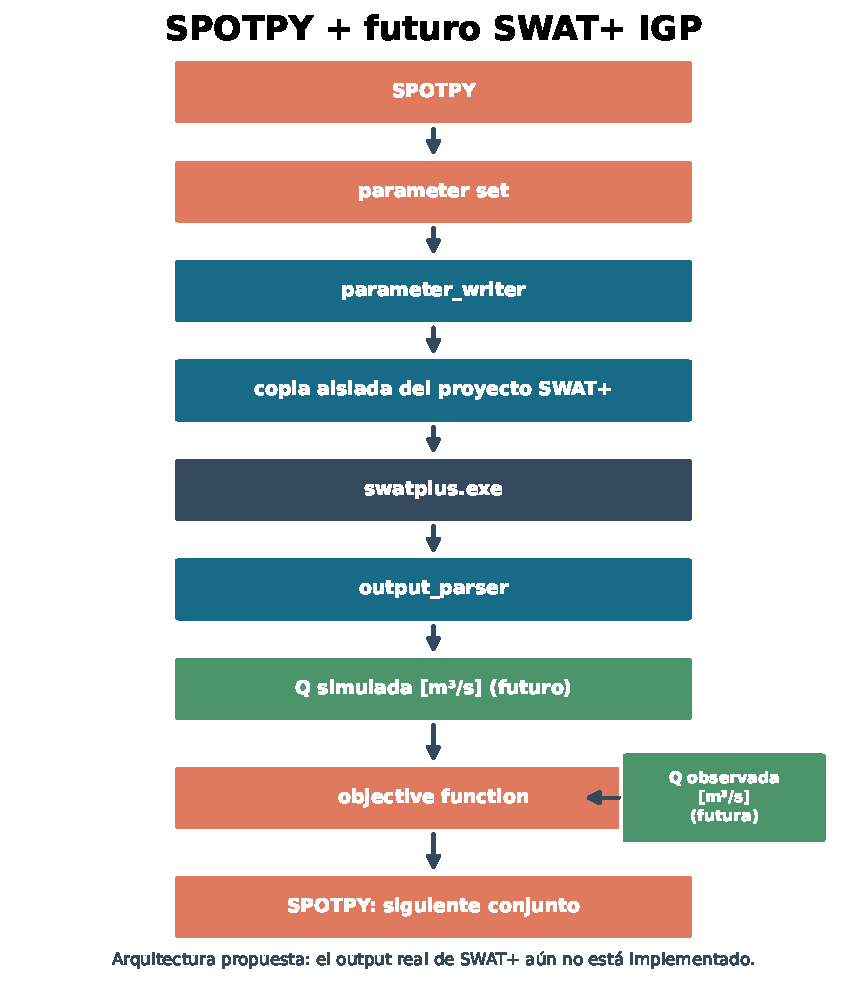
\includegraphics[width=.92\textwidth,height=.78\textheight,keepaspectratio]{figures/spotpy_swatplus_workflow.pdf}
\caption{Arquitectura propuesta; no representa una ejecución SWAT+ ya implementada.}\label{fig:swat}
\end{figure}

Faltan para integración real: ejecutable/version exacta; copia controlada del proyecto; parámetros, archivos y semántica de modificación; archivo/columna de caudal; unidades; estación y calendario; warm-up; reinicio; baseline; manejo de fallos y concurrencia. La Q futura se desea en m³/s, pero el laboratorio actual no define la unidad de \texttt{q\_obs}.

Cada worker debe poseer una copia mutable independiente. Compartir un proyecto produce carreras, outputs mezclados y corrupción. Se debe verificar primero una sola corrida secuencial y su reproducibilidad bit a bit o dentro de tolerancia documentada.
